
\documentclass{article}% use option titlepage to get the title on a page of its own.
\usepackage{cite}
\usepackage{listings}
\usepackage{color}
\usepackage{graphicx}
\usepackage{enumitem}


\definecolor{dkgreen}{rgb}{0,0.6,0}
\definecolor{gray}{rgb}{0.5,0.5,0.5}
\definecolor{mauve}{rgb}{0.58,0,0.82}

\lstset{frame=tb,
  language=Python,
  aboveskip=3mm,
  belowskip=3mm,
  showstringspaces=false,
  columns=flexible,
  basicstyle={\small\ttfamily},
  numbers=none,
  numberstyle=\tiny\color{gray},
  keywordstyle=\color{blue},
  commentstyle=\color{dkgreen},
  stringstyle=\color{mauve},
  breaklines=true,
  breakatwhitespace=true,
  tabsize=3
}
\begin{document}

\begin{titlepage}
	\begin{center}
	\line(1,0) {300} \\
	\huge{\textbf{Optimizaci\'on de Flujo en Redes: Reporte 3 }}
	\line(1,0) {300}\\
	
	\textsc{ \Large Mayra Cristina Berrones Reyes.  6291}\\ 
	\textsc{\Large Abril 2018} \\
	\end{center}
\end{titlepage}

\section*{Introducci\'on}

En este reporte se toman prestados los resultados de los grafos construidos en el Reporte2, \cite{reporte} en donde se realizaron grafos simples, dirigidos y ponderados. En este caso se tomaron dos tipos de algoritmos de alcance, y se pusieron en pr\'actica en de los caminos que existen dentro de los vertices de los grafos, tanto para ver como es su funcionamiento, como para verificar la eficiencia que tiene cada uno de ellos.


\begin{description}[font=$\bullet$~\normalfont\scshape\color{black}]
\item[\textbf{Floyd Warshall } ]

\end{description}

 Floyd-Warshall es un algoritmo b\'asico de alcance que adem\'as computa los caminos mas cortos si nuestro grafo es ponderado. El algoritmo se construye de una manera incremental, en donde se hacen estimaciones de los caminos m\'as cortos entre dos v\'ertices hasta llegar a la soluci\'on \'optima \cite{elisa}.
 \\
 
\begin{lstlisting}
// exp2.py
def floyd_warshall (self): 
		d = {}
		for v in self.V:
			d[(v, v)] = 0 # distancia reflexiva es cero
			for u in self.vecinos[v]: # para vecinos, la distancia es el peso
				if (v, u) in self.E:
					d[(v, u)] = self.E[(v, u)]
				else:
					d[(v, u)] = self.E[(u, v)]
		for intermedio in self.V:
			for desde in self.V:
				for hasta in self.V:
					di = None
					if (desde, intermedio) in d:
						di = d[(desde, intermedio)]
					ih = None
					if (intermedio, hasta) in d:
						ih = d[(intermedio, hasta)]
					if di is not None and ih is not None:
						c = di + ih # largo del camino via "i"
						if (desde, hasta) not in d or c < d[(desde, hasta)]:
							d[(desde, hasta)] = c # mejora al camino actual
		with open("Warshall.dat", "at") as archivo:
			print(d, file = archivo)
		return d
	
\end{lstlisting}

Para su complejidad vemos que el algoritmo tiene tres ciclos de \textit{for} por lo que su complejidad se va a $O(V)^3$. Este tipo de algoritmo es completamente dependiente de los n\'umeros de vertices de los grafos, por lo que lo hace especialmente util para ciertos tipos de grafos, mientras que en otros esto no nos ayuda en mucho \cite{floyd2}.


La pregunta que se puede formular es si el algoritmo Floyd-Warshall es bueno para los algoritmos que contienen muchas aristas conectando sus vertices, o uno de pocas aristas. La respuesta seria en un grafo con mas aristas, ya que el objetivo de este algoritmo es encontrar los caminos mas cortos que pueda unir todos los pares de vertices\cite{floyd1}. 


\begin{description}[font=$\bullet$~\normalfont\scshape\color{black}] 
\item[\textbf{Ford Fulkerson} ]

\end{description}

En el caso del algoritmo de Ford-Fulkerson nos inclinamos mas sobre el tema de flujos y cortes, que son problemas muy comunes dentro de los grafos ponderados. En este caso, tenemos dos vertices especiales, que llamamos \textbf{fuente} \textit{s} y \textbf{sumidero} \textit{t}. \cite{elisa}


En una forma r\'apida de explicarlo, tenemos que encontrar el camino que nos lleve del v\'ertice \textit{s} al v\'ertice \textit{t}, pasando por sus conexiones o aristas, las cuales tienen diferentes pesos o capacidades. Si nuestro grafo es dirigido, los valores en sentido contrario a la direcci\'on que se indica se vuelven negativos\cite{ford}. Esta es una manera bastante simplificada de como funciona el algoritmo, pero nos ayudar\'a a entender suficiente para saber lo que hace nuestro c\'odigo.

\begin{lstlisting}
// exp2.py
	def camino(self): #construccion de camino aumentante
		cola = [self.s]
		usados = set()
		camino = dict()
		while len(cola) > 0:
			u = cola.pop(0)
			usados.add(u)
			for (w, v) in self.E:
				if w == u and v not in cola and v not in usados:
					actual = self.f.get((u, v), 0)
					dif = self.E[(u, v)] - actual
					if dif > 0:
						cola.append(v)
						camino[v] = (u, dif)
		if self.t in usados:
			return camino
		else: # no se alcanzo
			return None	
\end{lstlisting}

Para poder utilizar el algoritmo de Ford-Fulkerson, primero tenemos que realizar un camino posible del v\'ertice \textit{s} al v\'ertice \textit{t}. Mientras existan mas caminos, el algoritmo los va a seguir comparando, hasta encontrar el que tenga menor peso, en nuestro caso.

\begin{lstlisting}
// exp2.py
	def ford_fulkerson(self): 
		self.s = self.P[2]
		self.t = self.P[randint(1, self.n - 1)][2]
		if self.s == self.t:
			return 0; #O puedes poner mensaje de que start and target son iguales.
		maximo = 0
		self.f = dict()
		while True:
			aum = self.camino()
			if aum is None:
				break #ya no hay
			incr = min(aum.values(), key = (lambda k: k[1]))[1]
			u = self.t
			while u in aum:
				v = aum [u][0]
				actual = self.f.get((v, u), 0) #cero si no hay
				inverso = self.f.get((u, v), 0)
				self.f[(v, u)] = actual + incr
				self.f[(u, v)] = inverso - incr
				u = v
			maximo += incr
		with open("Fulkerson.dat", "at") as archivo:
			print(maximo, file = archivo)
		return maximo
\end{lstlisting}

\section*{An\'alisis de los Algoritmos.}

Para poder hacer un an\'alisis del runtime de los algoritmos dependiendo de la cantidad de vertices y de aristas, se modific\'o el c\'odigo \textit{test.py} que se realiz\'o en el reporte anterior \cite{reporte} para poder tomar los tiempos de corrida con diferente cantidad de nodos, al igual que con diferentes grafos, dirigidos y no dirigidos.

\begin{lstlisting}
//test.py

import time
from exp2 import Grafo
puntos = 10
di = 3
proba = 0.5

if di > 2:
	for n in range(1, 21):
		for j in range(0, 10):
			if di is 3:
				with open("TiempoNoDir.csv", "at") as salida:
					tim = time.clock()
					i = 5 * n
					p = Grafo()
					p.puntos(i)
					p.conecta(proba, di)
					p.ford_fulkerson()
					p.floyd_warshall()
					p.imprimir("nodos.dat")
					p.grafica(di)
					print(time.clock() - tim, file = salida)

			elif di is 4:
				with open("TiempoDir.csv", "at") as salida:
					tim = time.clock()
					i = 5 * n
					p = Grafo()
					p.puntos(i)
					p.conecta(proba, di)
					p.ford_fulkerson()
					p.floyd_warshall()
					p.imprimir("nodos.dat")
					p.grafica(di)
					print(time.clock() - tim, file = salida)
\end{lstlisting}

\begin{figure*}[h!] 
\includegraphics[width = 1\textwidth]{Nodos2.eps}
\caption{Dirigido y ponderado.}
\label{td}
\end{figure*}
\break
\begin{figure*}[h!] 
\includegraphics[width = 1\textwidth]{Nodos3.eps}
\caption{Ponderado, sin direccion}
\label{td}
\end{figure*}

\break

\begin{figure*}[h!] 
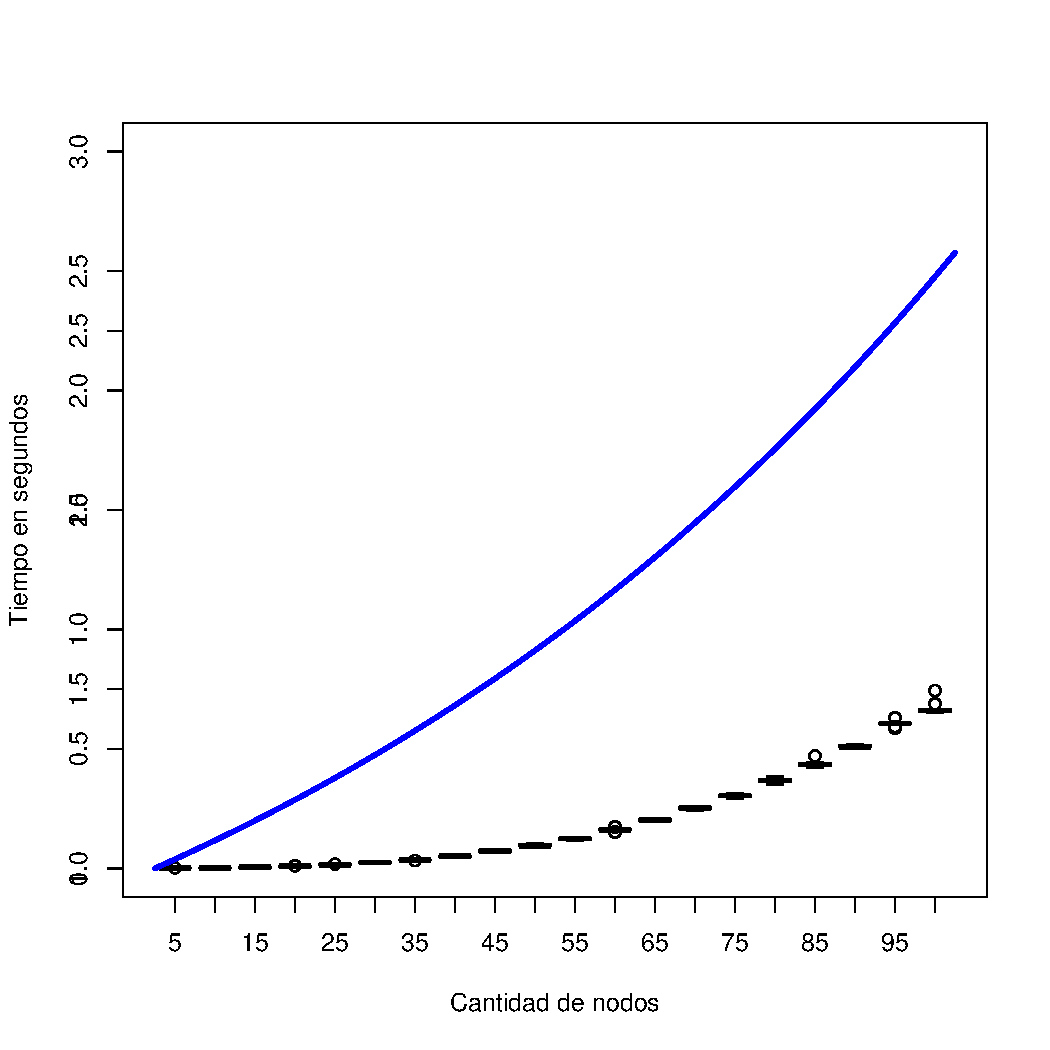
\includegraphics[width = 1\textwidth]{TiempoNoDirFinal.pdf}
\caption{Tiempo no dirigido}
\label{tnd}
\end{figure*}
\break
\begin{figure*}[h!] 
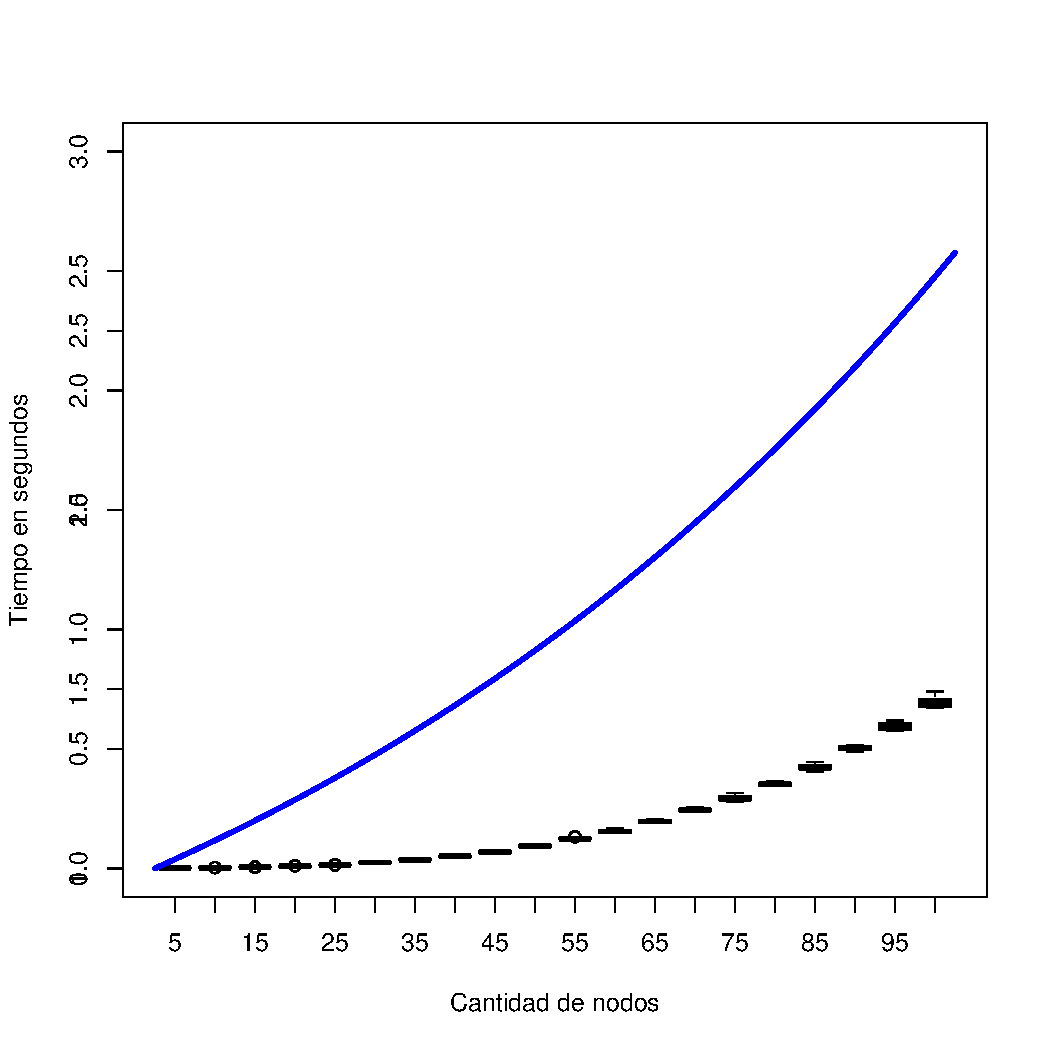
\includegraphics[width = 1\textwidth]{TiempoDirFinal.pdf}
\caption{Tiempo dirigido}
\label{td}
\end{figure*}

\break


\section*{Conclusi\'on}

Para finalizar, si se realiza una revisi\'on de las gr\'aficas resultantes, podemos ver que el tiempo de ejecuci\'on si aumenta de manera significativa. En la gr\'afica que se muestra en este reporte solamente llegamos a analizar 95 nodos, y la curva que se hizo si se pronunci\'o. En casos reales, supongo que no se van a utilizar una menor cantidad de 1000 nodos, lo cual podr�a costar bastante trabajo computacional.

Este reporte fue una buena introducci�n para los distintos algoritmos de alcance que existen, y cual es su funcionamiento, ya que en otras clases de optimizaci\'on se ha iniciado el estudio de este tipo de grafos, cortes y caminos, pero poderlos aterrizar a manera de algoritmos, ha ayudado a su mejor entendimiento.


\begin{thebibliography}{5}
\bibitem{reporte} \textsc{Berrones Reyes, Mayra Cristina} \textit{Reporte2. Marzo 2018}
\bibitem{elisa} \textsc{Schaeffer, Elisa} \textit{https://elisa.dyndns-web.com/teaching/mat/discretas/md.html} \textsc{Matem\'aticas Discretas. Grafos y \'arboles.}  \textbf{Retrieved. Abril. 2018}
\bibitem{floyd2} \textsc{Floyd-Warshall Algorithm.} \textit{Brilliant.org, from https://brilliant.org/wiki/floyd-warshall-algorithm/} \textbf{Retrieved. April 3. 2018}
\bibitem{floyd1}\textsc{Michael Sambol} \textit{Step by step instructions showing how to run the Floyd?Warshall algorithm on a graph.} \textit{Publicado. 16 Julio. 2016, from https://www.youtube.com/watch?v=4OQeCuLYj-4}
\bibitem{ford} \textsc{Michael Sambol} \textit{Ford-Fulkerson in 5 minutes ? Step by step example} \textit{Publicado 7 de Julio 2016, from https://www.youtube.com/watch?v=Tl90tNtKvxs}

\end{thebibliography}

\end{document} 












